\section{Testing}
\subsection{Analisi statica}
Per l'analisi statica del codice Java è stato utilizzato il tool STAN4J, integrato nel IDE Eclipse.

\subsection{Analisi dinamica}
Nell'iterazione 3 si sono testate tutte le API Rest implementate, utlizzando Postman (\Fig \ref{fig:RisultatiTestAPIIT3}). In particolare si sono testate le seguenti funzionalità:

\begin{itemize}
	\item AreaController:
	\begin{itemize}
		\item Visualizzazione degli ultimi dati meteo scaricati di un'area, il cui id è specificato nel oath della richiesta;
		\item Visualizzazione del più recente allarme relativo a nebbia o brina associata all'area il cui id è specificato nel path della richiesta;
	\end{itemize}

	\begin{figure}[h!]
		\centering
		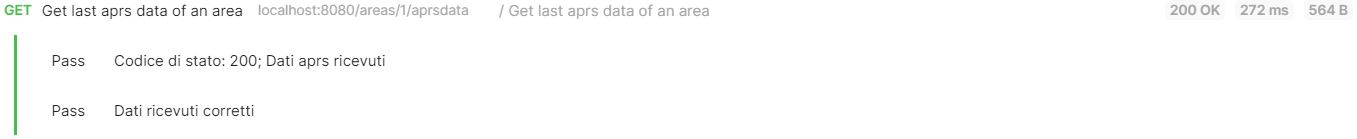
\includegraphics[width=1\linewidth]{./Iterazione 3/ImageFiles/TestGetAprsData}
		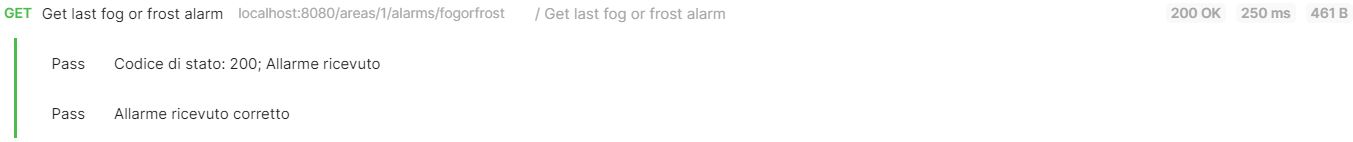
\includegraphics[width=1\linewidth]{./Iterazione 3/ImageFiles/TestGetFrostOrFogAlarm}
		\caption{Risultati test API su Postman.}
		\label{fig:RisultatiTestAPIIT3}
	\end{figure}
\end{itemize}

\clearpage

\subsection{Unit Test}
\subsubsection{LvsEmergency Server}
In questa iterazione è stata testata la funzione \textit{findFirstByAprsDataIdNameOrderByAprsDataIdTimeDesc(String name)} che recupera i dati più recenti relativi alla stazione APRS, il cui \textit{name} è specificato nel parametro. Di seguito è riportato il codice del test.

\lstinputlisting[language=Java]{./Iterazione 3/OtherFiles/AprsDataRepositoryTest.java}

Il risultato del test con JUnit ha confermato il corretto funzionamento della funzione.

\begin{figure}[h!]
	\centering
	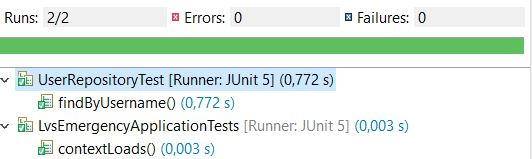
\includegraphics[width=0.6\linewidth]{./Iterazione 3/ImageFiles/TestJUnit}
	\caption{Risultato test con JUnit.}
	\label{fig:RisultatiTestJunitIT3}
\end{figure}

\clearpage

\subsubsection{Client App}
Lato client è stata testata la corretta creazione delle classi inserite nell'iterazione 3, \texttt{AprsData} e \texttt{Alarm} a partire da una stringa Json. Di seguito è riportato il codice del test: 

\lstinputlisting[language=C++]{./Iterazione 3/OtherFiles/testcpp.txt}

Il risultato dei test ha confermato il corretto funzionamento delle nuove funzioni e di quelle precedenti. 

\begin{figure}[h!]
	\centering
	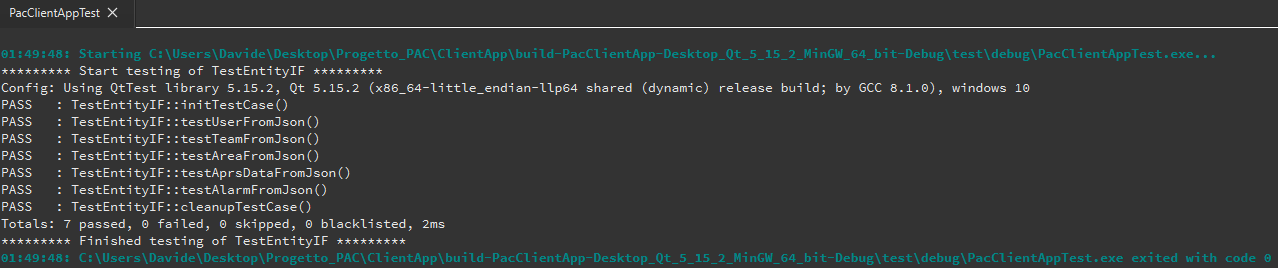
\includegraphics[width=1\linewidth]{./Iterazione 3/ImageFiles/testQt}
	\caption{Risultato test con Qt Test.}
	\label{fig:RisultatiTestQtIT3}
\end{figure}
\clearpage

\subsection{Documentazione API}

In questa sezione viene mostrata la documentazione relativa ad alcune API implementate nell'iterazione 3. \`E possibile visualizzare una collezione (creata con Postman) di tutte le API realizzate e testate sulla repository GitHub. In particolare, si riportano di seguito le più significative:
\begin{itemize}
	\item API per la visualizzazione degli ultimi dati meteorologici raccolti dalla stazione APRS associata all'area, il cui id è specificato nel path della richiesta;
	\item API per la visualizzazione del più recente allarme di nebbia o brina generato nell'area di interesse;
\end{itemize}

\begin{figure}[h!]
	\centering
	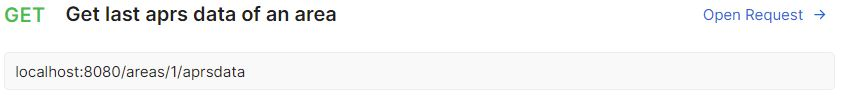
\includegraphics[width=1\linewidth]{./Iterazione 3/ImageFiles/GetAprsDataRequest}
	\lstinputlisting[language=json]{./Iterazione 3/OtherFiles/GetAprsDataResponse.json}
	\caption{Documentazione API Get Aprs data.}
	\label{fig:LoginAPI}
\end{figure}

\begin{figure}[h!]
	\centering
	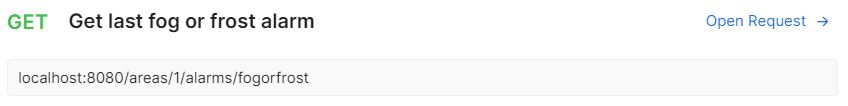
\includegraphics[width=1\linewidth]{./Iterazione 3/ImageFiles/GetFrostOrFogAlarmRequest}
	\lstinputlisting[language=json]{./Iterazione 3/OtherFiles/GetFrostOrFogAlarmResponse.json}
	\caption{Documentazione API Get fog or frost alarm.}
	\label{fig:GetOneUserAPI}
\end{figure}
